%-----------------------------------------------------------------
%	PERFORMANCE
%	!TEX root = ./../main.tex
%-----------------------------------------------------------------
\section{Assessment of the solution}\label{sec:assessment}

%-----------------------------------------------------------------
\subsection{Analysis with TAU}

Up to this point we are well aware of how the performance increases using OpenMP as a tool to parallelise the code. So now we want to explore further parallelisation, but using MPI this time. Once again we are going to use TAU, a toolkit for analysis performance that allows us to study in detail the performance of many parts of the code that we have parallelised.

As a comparison, we have used the same code as before with the same number of iterations and problem size.

%-----------------------------------------------------------------
\subsection{Influence of the number of threads}

%-----------------------------------------------------------------
\subsubsection{Using profile files (\texttt{paraprof})}

The toolkit \inline{paraprof} (bundled with TAU) allows us to parallel profile analysis. This is similar to using \inline{perf stat}, but now we have data for each of the threads.

For this part, we need to set the following environment variable:
\begin{lstlisting}
export TAU_PROFILE=1
\end{lstlisting}

Then we have to compile our source code using TAU, and then run it as usual
\begin{lstlisting}
tau_cc.sh -lm laplaceMPI.c -o mpiruntau
mpirun -np N ./mpiruntau 512 500
\end{lstlisting}
where \inline{N} can be 2 or 4.

This will give us \inline{profile.0.0.*} profile files; one for each of the threads used. To read and analyse these files we can use the \inline{paraprof} tool.

\bigskip

The result of the execution of the program using 2 and 4 threads can be seen in the tables \ref{tab:paraprof2}, \ref{tab:paraprof4} and figures \ref{fig:paraprof2-heat}, \ref{fig:paraprof4-heat} below. They show quite interesting results. On one hand we can see how the \emph{Run Time} of execution of the internal MPI operations are pretty much the same. The only main difference is the execution of the whole program itself; this is the calculation of the Laplace step.

An interesting conclusion that can be extracted from these graphs is that all threads are performing more or less the same. This is reflected in the fact we can not appreciate a big difference in the time needed for every thread; they all took the same time to finish the same work. This would be completely different if we have assigned a specific thread to act as a master only, instead of the master doing calculations as well.

\begin{table}[H]
    \centering
    \begin{tabular}{l c c}
        \toprule
        \toprule
        \textbf{Function} & \textbf{Thread 0}    & \textbf{Thread 1} \\
        \midrule
        \texttt{MPI\_Init()}       & \num{283}   & \num{282}   \\
        \texttt{MPI\_Comm\_size()} & \num{0}     & \num{0}     \\
        \texttt{MPI\_Comm\_rank()} & \num{0}     & \num{0.001} \\
        \texttt{MPI\_Send()}       & \num{0.877} & \num{1}     \\
        \texttt{MPI\_Recv()}       & \num{47}    & \num{50}    \\
        \texttt{MPI\_Finalize()}   & \num{81}    & \num{81}    \\
        \texttt{.TAU application}  & \num{7139}  & \num{7138}  \\
        \bottomrule
    \end{tabular}
    \caption{Run time (in ms) obtained on 2 threads}
    \label{tab:paraprof2}
\end{table}

\begin{figure}[H]
	\centering
	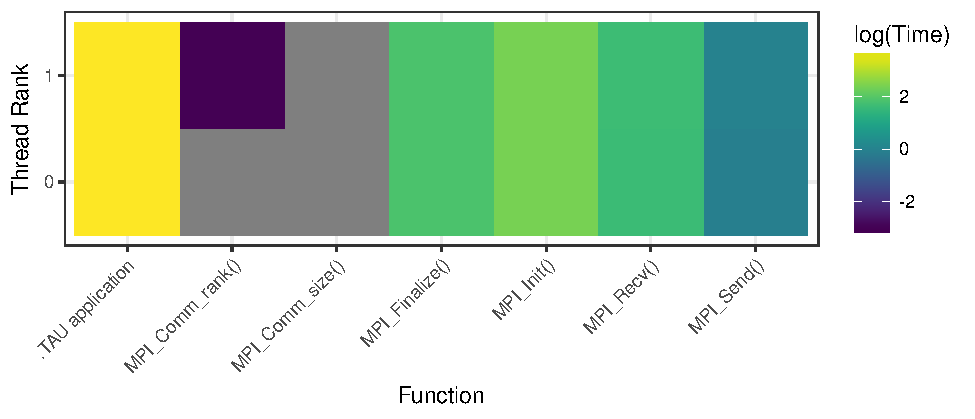
\includegraphics[width=0.95\textwidth]{images/pprof-2}
	\caption{Heatmap of the run time (in ms) obtained on 2 threads}
	\label{fig:paraprof2-heat}
\end{figure}

\begin{table}[H]
    \centering
    \begin{tabular}{l c c c c}
        \toprule
        \toprule
        \textbf{Function} & \textbf{Thread 0} & \textbf{Thread 1} & \textbf{Thread 2} & \textbf{Thread 3} \\
        \midrule
        \texttt{MPI\_Init()}       & \num{298}  & \num{284}  & \num{281}  & \num{276}  \\
        \texttt{MPI\_Comm\_size()} & \num{0}    & \num{0}    & \num{0}    & \num{0}    \\
        \texttt{MPI\_Comm\_rank()} & \num{0}    & \num{0}    & \num{0}    & \num{0}    \\
        \texttt{MPI\_Send()}       & \num{1}    & \num{1}    & \num{1}    & \num{1}    \\
        \texttt{MPI\_Recv()}       & \num{60}   & \num{28}   & \num{34}   & \num{55}   \\
        \texttt{MPI\_Finalize()}   & \num{81}   & \num{81}   & \num{82}   & \num{82}   \\
        \texttt{.TAU application}  & \num{3809} & \num{3795} & \num{3793} & \num{3788} \\
        \bottomrule
    \end{tabular}
    \caption{Run time (in ms) obtained on 4 threads}
    \label{tab:paraprof4}
\end{table}

\begin{figure}[H]
	\centering
	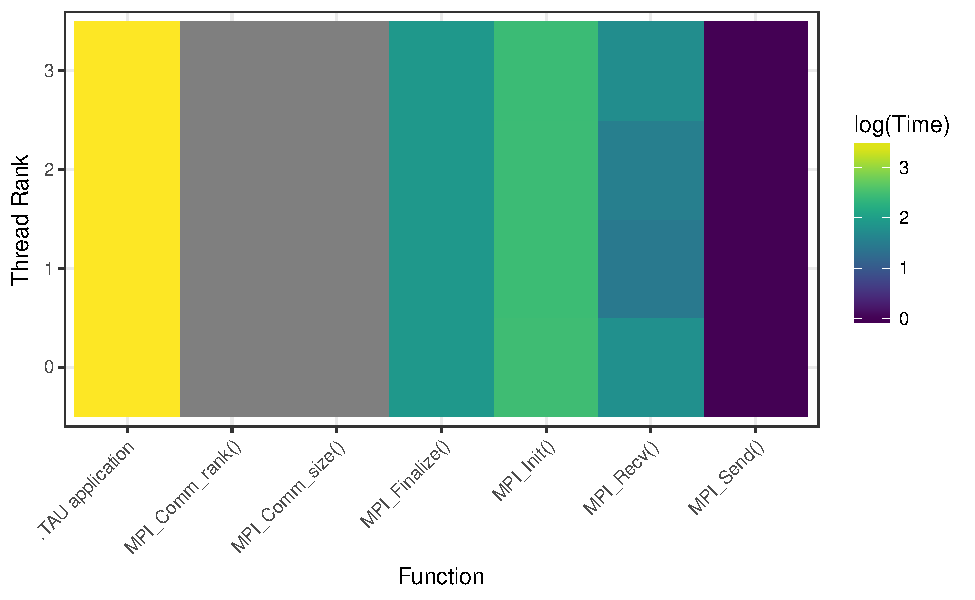
\includegraphics[width=0.95\textwidth]{images/pprof-4}
	\caption{Heatmap of the run time (in ms) obtained on 4 threads}
	\label{fig:paraprof4-heat}
\end{figure}

We can see that the time of this distributed version using MPI is $T/N + $ communication-overhead (where $T$ is the time it takes for the sequential algorithm to complete). Using 4 threads instead of 2 does not give us exactly half the compilation time; we get $\approx \SI{3800}{ms}$ instead of $\approx \SI{7100/2}{ms} = \SI{3550}{ms}$.

%-----------------------------------------------------------------
\subsubsection{Using traces (\texttt{jumpshot})}

Now that we have seen some of the standard measurement tools for parallelised code, we can explore even more detailed analytical tools. 

In particular, we aim to see the relations established between the threads and the information they process. This analysis could lead to a better insight on the strengths and weaknesses of our parallelisation and facilitate further improvement. 

In order to do so, we must first to arrange some technical issues.

First of all, we need to set the following environment variable:
\begin{lstlisting}
export TAU_TRACE=1
\end{lstlisting}

Then we have to compile our source code using TAU, and then run it as usual
\begin{lstlisting}
tau_cc.sh -lm laplaceMPI.c -o mpiruntau_trace
mpirun -np N ./mpiruntau_trace 512 500
\end{lstlisting}
where \inline{N} can be 2 or 4.

After doing this, we have to merge the obtained \inline{tautrace.0.0.*.trc} trace files into a readable \inline{.slog2} log file using the following commands:
\begin{lstlisting}
tau_treemerge.pl
tau2slog2 tau.trc tau.edf -o tauNthreads.slog2
\end{lstlisting}

To visualise the data of the logfile, we simply use the \inline{jumpshot} tool (also bundled with TAU):
\begin{lstlisting}
jumpshot tauNthreads.slog2
\end{lstlisting}

\bigskip

In figures \ref{fig:jumpshot2} and \ref{fig:jumpshot4} we can see an example of the Time Line of internal operations of each one of the used threads. Essentially, it shows us the information exchanged between different threads in chronological order. This helps us to understand how information/messages are sent and recieved by the different threads to perform the parallelisation. 

One crucial point of this visualisation is to spot redundancies or any kind of misperformance within the code.

\begin{figure}[H]
	\centering
	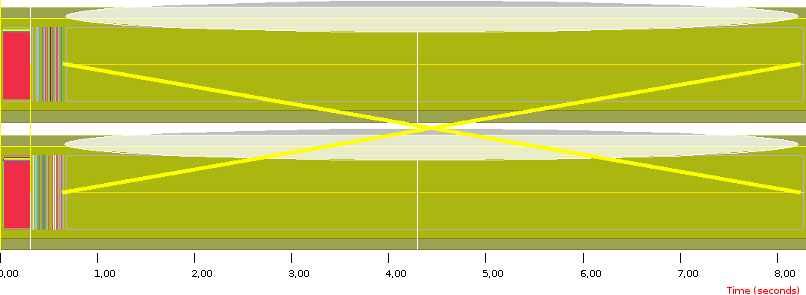
\includegraphics[width=0.85\textwidth]{images/trace2b}
	\caption{Time Line of the 2 threads using \inline{jumpshot}}
	\label{fig:jumpshot2}
\end{figure}

\begin{figure}[H]
	\centering
	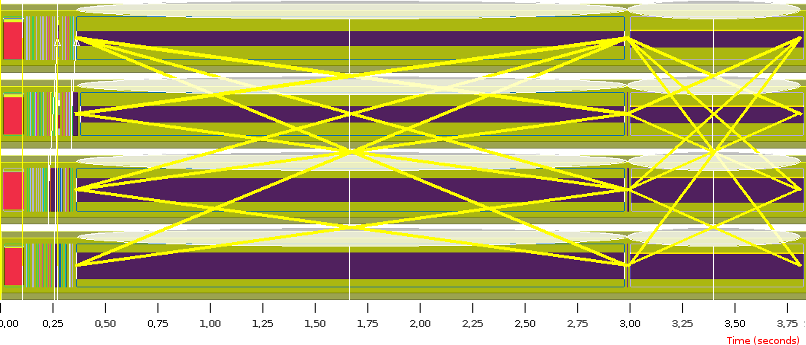
\includegraphics[width=0.85\textwidth]{images/trace4c}
	\caption{Time Line of the 4 threads using \inline{jumpshot}}
	\label{fig:jumpshot4}
\end{figure}

It is interesting to notice how the work is distributed and iteratively reorganised along the different threads within the timeline of the computation.

%-----------------------------------------------------------------
\subsection{Influence of the problem size}

%-----------------------------------------------------------------
\subsubsection{Using profile files (\texttt{paraprof})}

Up until now, we have learnt how our code behaves when different degrees of parallelisation are applied. Moreover, we now know some of the internal details involved in the performance of our new optimised code. 

One question that we now could ask ourselves is how the performance of the code scales. Until now we have studied the increase in the performance for a given magnitude of the matrix, but we have not considered how a change in this magnitude could affect the the computational effort needed to solve it. At first sight, we could guess that the larger the size of the matrix, the longer it will take to finish the problem. But, would all functions within the code increase in the same way? Or some functions would be more affected than others?

One way to address these questions and evaluate the scalability is simply to run the code for different matrix sizes and measure the time needed each time.

For this part, we need to set the following environment variables:
\begin{lstlisting}
export TAU_PROFILE=1
export TAU_TRACE=0
\end{lstlisting}

Then we have to compile our source code using TAU, and then run it as usual
\begin{lstlisting}
tau_cc.sh -lm laplaceMPI.c -o mpiruntau
mpirun -np 4 ./mpiruntau n 500
\end{lstlisting}
where we have chosen \inline{n} to be 128, 256, 384, 512, 640, and 768.

\begin{table}[H]
    \centering
    \resizebox{\textwidth}{!}{%
    \begin{tabular}{l c c c c c c}
        \toprule
        \toprule
        \textbf{Function} & $\mathbf{128 \times 128}$ & $\mathbf{256 \times 256}$ & $\mathbf{384 \times 384}$ & $\mathbf{512 \times 512}$ & $\mathbf{640 \times 640}$ & $\mathbf{768 \times 768}$ \\
        \midrule
        \texttt{MPI\_Init()}       & \num{287}     & \num{334}  & \num{284}     & \num{281}    & \num{280}     & \num{281}     \\
        \texttt{MPI\_Comm\_size()} & \num{0.0005}  & \num{0}    & \num{0.00025} & \num{0.0005} & \num{0.00075} & \num{0.0005}  \\
        \texttt{MPI\_Comm\_rank()} & \num{0.00025} & \num{0}    & \num{0}       & \num{0}      & \num{0.00025} & \num{0.00025} \\
        \texttt{MPI\_Send()}       & \num{0.583}   & \num{1}    & \num{1}       & \num{1}      & \num{1}       & \num{2}       \\
        \texttt{MPI\_Recv()}       & \num{7}       & \num{15}   & \num{12}      & \num{13}     & \num{13}      & \num{13}      \\
        \texttt{MPI\_Finalize()}   & \num{82}      & \num{282}  & \num{81}      & \num{82}     & \num{82}      & \num{119}     \\
        \texttt{.TAU application}  & \num{600}     & \num{1618} & \num{2299}    & \num{3781}   & \num{5483}    & \num{7705}    \\
        \bottomrule
    \end{tabular}}
    \caption{Run time (in ms) obtained on 4 threads for different problem sizes}
    \label{tab:paraprof-sizes}
\end{table}

\begin{figure}[H]
	\centering
	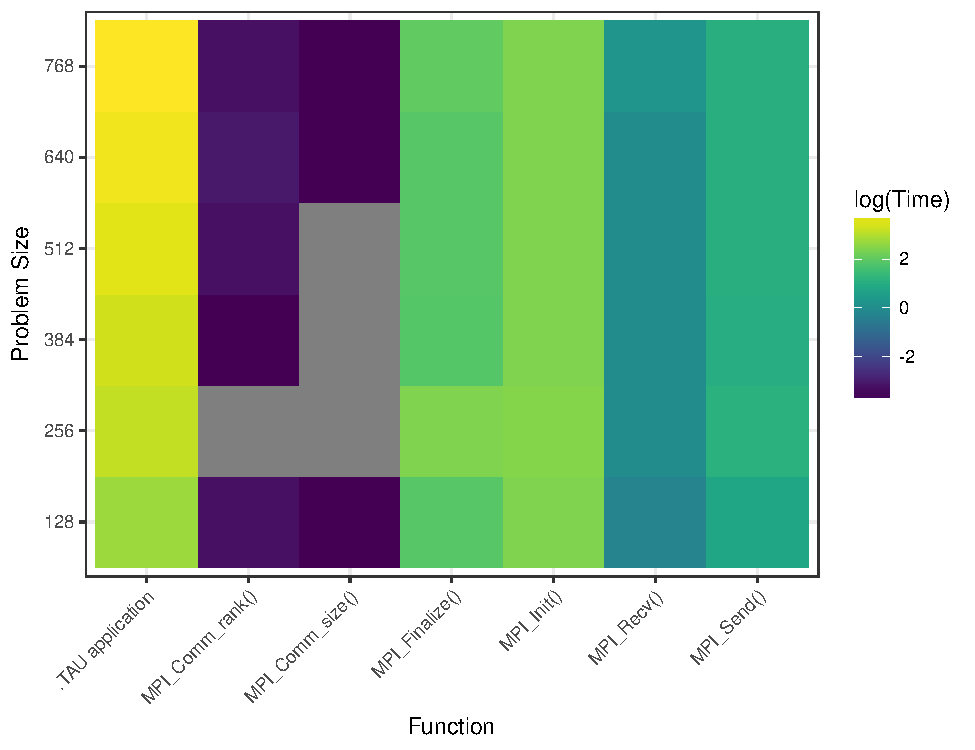
\includegraphics[width=0.95\textwidth]{images/pprof-sizes}
	\caption{Heatmap of the mean run time (in ms) obtained on 4 threads for different problem sizes}
	\label{fig:paraprof-sizes-heat}
\end{figure}

A possible concern involving the usage of MPI could be the loss of efficiency caused by the constant interchange of information between the threads. This loads more work to our code and thus can slow down the final output of the code, even though we aim to increase the performance thanks to making some processes parallel. We have checked that this not happens for a matrix where $n = 512$, because the improvement caused thanks to the parallelisation largely overcomes the possible lack of performance that more lines of orders could cause. Then, a still reasonable concern would be asking whether the parallelisation is also worth it for different dimensions of the problem. 

Table \ref{tab:paraprof-sizes} shows how the time needed to execute our program increases over the size of the problem. Looking at figure \ref{fig:paraprof-sizes-heat}, we can visualise and distinguish where this increase in time is happening; and notice that the function \inline{.TAU application} is the one suffering an increase in time execution, whereas all others increase are clearly negligible, if existent. That function is the one responsible for the computations of the matrix, whilst the others are those MPI functions needed to exchange information between the different threads.

Every possible drawback is, then, absolutely dwarfed by the increase in the performance caused by the parallelisation method that we have implemented. And this effect becomes even greater when we increase the size of the problem.
